\documentclass[tikz]{standalone}
\tikzset{
  >=latex
}

\begin{document}
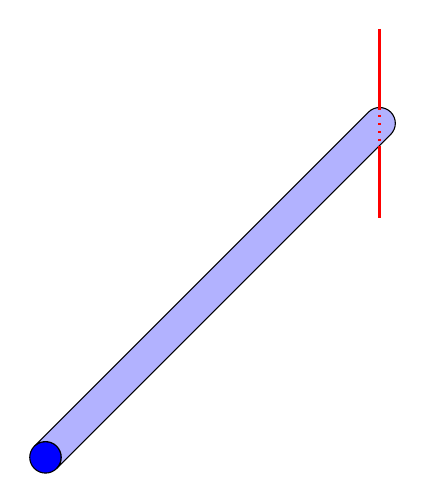
\begin{tikzpicture}[rotate=45]
  \draw[fill=blue] (0,0) circle (.2);
  \draw[fill=blue!30] (0,.2)--(6,.2) arc (90:-90:.2)--(0,-.2) arc(-90:90:.2);
  \draw[thick,red,rotate around={-45:(6,0)}] (6,1.2)--(6,.2);
  \draw[thick,red,dotted,rotate around={-45:(6,0)}] (6,.2)--(6,-.29);
  \draw[thick,red,rotate around={-45:(6,0)}] (6,-.29)--(6,-1.2);
%  \fill[red] circle (.03);
%  \draw[thick,red] (-1,0)--(0,0);
%  \draw[thick,red,dashed] (0,0)--(5.3,0);
%  \draw[thick,red] (5.3,0)--(5,0);
\end{tikzpicture}
\end{document}
